\documentclass[12pt]{article}
\usepackage[a4paper]{geometry}
\usepackage{fullpage}
\usepackage[T1]{fontenc}
\usepackage[utf8]{inputenc}
\usepackage{graphicx}
\usepackage{mathpazo}
\pagenumbering{gobble}
\usepackage{siunitx}
\DeclareSIUnit\voltampere{VA}
\usepackage{amsmath}
\usepackage[spanish]{babel}
\usepackage{steinmetz}
\usepackage{enumitem}
\renewcommand{\thesection}{Problema \arabic{section}}

\begin{document}

\title{}

\date{}

\section{}
En el circuito de la figura los valores se dan en voltios y ohmios, según corresponda. Determinar el valor de la intensidad I aplicando la propiedad de proporcionalidad.

\begin{center}
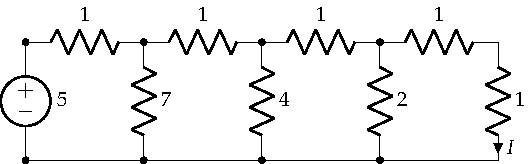
\includegraphics{../figs/problema_proporcionalidad}
\end{center}

\noindent\hrulefill

Suponiendo que $I = \SI{1}{\ampere}$, resolvemos el circuito hacia el generador. Obtenemos $\epsilon = \SI{11}{\volt}$. Por tanto, con un generador de $\SI{5}{\volt}$ la corriente será $I = \SI[parse-numbers=false]{5/11}{\ampere}$ (regla de tres simple).


\section{}

En el circuito de la figura determina:
\begin{itemize}
\item $u_R(t)$  y $u_L(t)$.
\item Balance de potencias.
\end{itemize}

\begin{center}
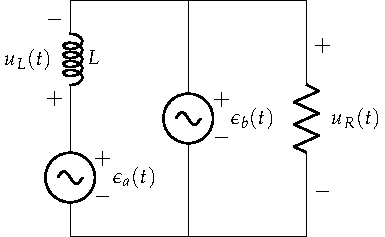
\includegraphics{../figs/superposicion2_ej}
\end{center}


Datos:
\begin{align*}
  e_a(t) &= \SI[parse-numbers=false]{3\sqrt{2} \sin(10^3 t)}{\volt}\\
  e_b(t) &= \SI[parse-numbers=false]{30\sqrt{2} \sin(10^4 t)}{\volt}\\
  R &= \SI{30}{\ohm}\\
  L &= \SI{3}{\milli\henry}
\end{align*}


\noindent\hrulefill

\subsection*{Solución}

Dado que las fuentes trabajan a frecuencias diferentes, hay que resolver mediante superposición.

Activamos una de las fuentes:
\begin{center}
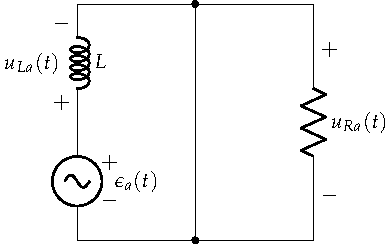
\includegraphics{../figs/superposicion2_A}
\end{center}

La resistencia está cortocircuitada. Por tanto:

\begin{align*}
  u_{Ra}(t) &= \SI{0}{\volt}\\
  u_{La}(t) &= \epsilon_a(t)\\  
\end{align*}

En este circuito la potencia disipada por la resistencia es $P_{Ra} = \SI{0}{\watt}$ y, en consecuencia, la potencia entregada por el generador es $P_{\epsilon_a} = \SI{0}{\watt}$.

Hacemos el análisis con la otra fuente:

\begin{center}
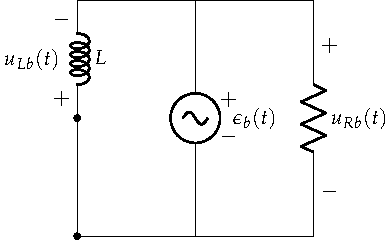
\includegraphics{../figs/superposicion2_B}
\end{center}

En este circuito:

\begin{align*}
  u_{Rb}(t) &= \epsilon_b(t)\\
  u_{Lb}(t) &= -\epsilon_b(t)\\  
\end{align*}

El balance de potencias es:

\begin{equation*}
  P_{Rb} = \frac{\epsilon_b^2}{R_b} = \SI{30}{\watt} = P_{\epsilon_b}\\
\end{equation*}

Por tanto:

\begin{align*}
  u_R(t) &= u_{Ra}(t) + u_{Rb}(t) = 30\sqrt{2}\sin(10^4 t)\\
  u_L(t) &= u_{La}(t) + u_{Lb}(t) = 3\sqrt{2}\sin(10^3 t) - 30\sqrt{2}\sin(10^4 t)\\
\end{align*}

Además, dado que las dos señales de los generadores son ortogonales, podemos sumar las potencias calculadas en cada circuito:

\begin{align*}
  P_R &= P_{Ra} + P_{Rb} = \SI{30}{\watt}\\
  P_\epsilon &= P_{\epsilon_a} + P_{\epsilon_b} = \SI{30}{\watt}\\
\end{align*}

\clearpage

\section{}

El circuito de la figura se encuentra en régimen permanente. Determina
analíticamente la expresión de $i(t)$, así como las potencias entregadas por los
generadores y disipadas por las resistencias $R_1$, y $R_2$.
\begin{center}
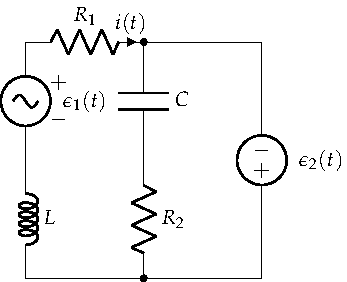
\includegraphics{../figs/superposicion1}
\end{center}

Datos:
\begin{align*}
  e_1(t) &= \SI[parse-numbers=false]{50 \sin(1000 t)}{\volt}\\
  e_2(t) &= \SI{30}{\volt}\\
  R_1 &= \SI{6}{\ohm}\\
  R_2 &= \SI{6}{\ohm}\\
  L &= \SI{8}{\milli\henry}\\
  C &= \SI{10}{\micro\farad}
\end{align*}


\noindent\hrulefill

\subsection*{Solución}

Aplicamos superposición.

Analizamos con la fuente de corriente alterna:

\begin{center}
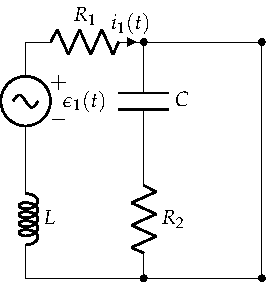
\includegraphics{../figs/superposicion1_AC}
\end{center}

La rama $R_2 - C$ está cortocircuitada y, por tanto, podemos prescindir de ella:

\begin{align*}
  \overline{Z}_1 &= R_1 + jX_L = 6 + 8j\si{\ampere}\\
  \overline{I}_1 &= \overline{\epsilon}_1 / \overline{Z}_1 = 5\sqrt{2}/2\phase{\ang{-53.13}}\si{\ampere}
\end{align*}

En el dominio del tiempo obtenemos:

\begin{equation*}
  i_1(t) = 5\sin(1000t - 0.9273)\si{\ampere}
\end{equation*}

En cuanto al balance de potencias:

\begin{align*}
  P_{R11} &= I_1^2 R_1 = \SI{75}{\watt}\\
  P_{R21} &= \SI{0}{\watt}\\
  P_{\epsilon_1} &= \Re(\overline{\epsilon}_1 \cdot \overline{I}_1^*) = \SI{75}{\watt}
\end{align*}

Analizamos con la fuente de corriente continua:

\begin{center}
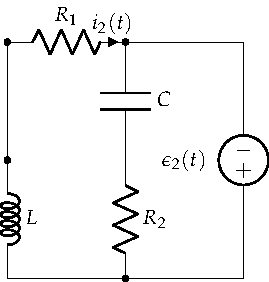
\includegraphics{../figs/superposicion1_DC}
\end{center}

En este circuito sustituimos la bobina por un cortocircuito y el condensador por un circuito abierto. En consecuencia:

\begin{equation*}
  i_2(t) = \epsilon_2(t) / R_1 = \SI{5}{\ampere}
\end{equation*}

En cuanto al balance de potencias:

\begin{align*}
  P_{R12} &= I_2^2 \cdot R_1 = \SI{150}{\watt}\\
  P_{R22} &= \SI{0}{\watt}\\
  P_{\epsilon2} &= \epsilon_2 \cdot I_2 = \SI{150}{\watt}
\end{align*}

Por tanto:

\begin{equation*}
  i(t) = i_1(t) + i_2(t) = 5 + 5\sin(1000t - 0.9273)\si{\ampere}
\end{equation*}

Además, como las señales son ortogonales, podemos hacer el balance de potencias conjunto con los dos circuitos:

\begin{align*}
  P_{R1} &= P_{R11} + P_{R12} = \SI{225}{\watt}\\
  P_{R2} &= P_{R21} + P_{R22} = \SI{0}{\watt}\\
  P_{\epsilon} &= P_{\epsilon1} + P_{\epsilon2} = \SI{225}{\watt}\\
\end{align*}

\clearpage

\section{}

En el circuito de la figura el generador de tensión $e(t)$ es de onda cuadrada simétrica, tal y como se muestra en la figura. La potencia total disipada por las resistencias $R_1$ y $R_2$ es de $\SI{40}{\watt}$.
Determina:

\begin{itemize}
  \item Valor máximo $E_0$ de la onda cuadrada.
  \item Forma de onda de la tensión $u(t)$ y su valor eficaz.
  \item Potencias disipadas en $R_1$ y $R_2$ si la frecuencia de la onda $e(t)$ aumenta al doble.
\end{itemize}

\begin{center}
  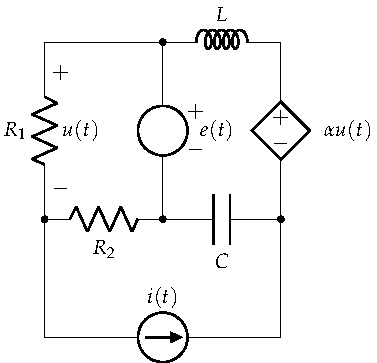
\includegraphics{../figs/superposicion3}
  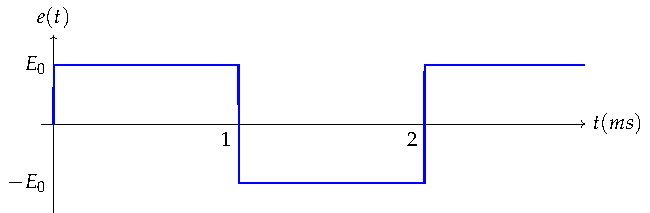
\includegraphics{../figs/superposicionOndaCuadrada}
\end{center}
Datos:

\begin{align*}
  i(t) &= \SI{1}{\ampere}\\
  R_1 &= \SI{60}{\ohm}\\
  R_2 &= \SI{40}{\ohm}\\
  L &= \SI{10}{\milli\henry}\\
  C &= \SI{1}{\micro\farad}
\end{align*}

\noindent\hrulefill

\subsection*{Solución}

Aplicamos superposición.

Activamos en primer lugar la fuente de corriente porque es de la que tenemos información completa para resolver.

\begin{center}
  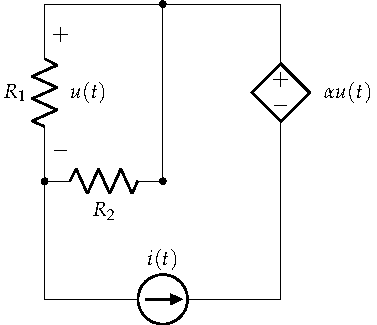
\includegraphics{../figs/superposicion3_DC}
\end{center}

Podemos sustituir las dos resistencias por su equivalente paralelo, $R_p = \SI{24}{\ohm}$, y calcular la potencia y la tensión:

\begin{align*}
  U_{Ig} &= I_g R_p = \SI{24}{\volt}\\
  P_{R_1R_2I_g} &= I_g^2 \cdot R_p = \SI{24}{\watt}
\end{align*}

Este último resultado podemos utilizarlo en el circuito de la otra fuente, porque las señales son ortogonales. Por tanto:

\begin{equation*}
  P_{R1R2} = P_{R1R2e} + P_{R1R2I_g} \rightarrow P_{R1R2e} = \SI{16}{\watt}
\end{equation*}

\begin{center}
  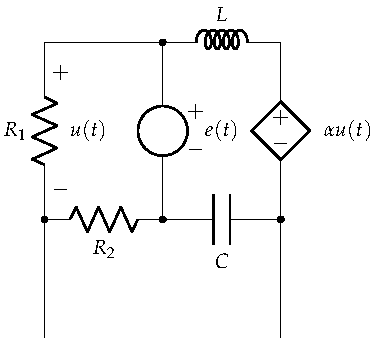
\includegraphics{../figs/superposicion3_fuentepulsos}
\end{center}

En este circuito la fuente está conectada en paralelo con la conexión serie de las dos resistencias. Así, la potencia disipada por las dos resistencias en este circuito es:

\begin{equation*}
  P_{R1R2e} = \frac{E^2}{R_1 + R_2} = \frac{E^2}{100} = \SI{16}{\watt} \rightarrow E = \SI{40}{\volt}
\end{equation*}

Teniendo en cuenta que en un tren de pulsos simétrico el valor eficaz, $E$, coincide con el valor máximo, $E_0$, obtenemos $E_0 = \SI{40}{\volt}$.

Por otra parte, en este circuito podemos obtener la tensión en la resistencia $R_1$ mediante un divisor de tensión:
\begin{equation*}
  u_e(t) = e(t) \cdot \frac{R_1}{R_1 + R_2} = 0.6\cdot e(t)
\end{equation*}

El resultado es un tren de pulsos simétrico con valor máximo $U_{e0} = \SI{24}{\volt}$.

Combinando los dos circuitos obtenemos:

\begin{equation*}
  u(t) = u_{Ig}(t) + u_e(t) = 24 + 0.6 \cdot e(t)
\end{equation*}

\begin{center}
  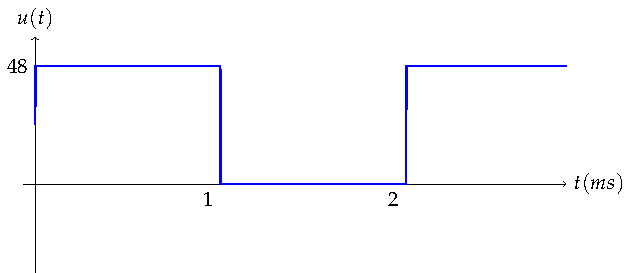
\includegraphics{../figs/superposicionOndaCuadrada2}
\end{center}

Para calcular el valor eficaz de esta señal podemos aplicar la definición:

\begin{align*}
  U &= \sqrt{\frac{1}{T}\int_0^Tu^2(t)\mathrm{d}t} = \\
    &= \sqrt{500 \int_0^{10^-3}48^2 \mathrm{d}t} = \\
  &= \SI[parse-numbers=false]{24\sqrt{2}}{\volt}
\end{align*}

También podemos aprovechar el hecho de que sean señales ortogonales:

\begin{equation*}
  P_{R1} = \frac{U^2}{R_1} = \frac{U_{Ig}^2}{R_1} + \frac{U_e^2}{R_1} \rightarrow U^2 = U_{Ig}^2 + U_e^2
\end{equation*}

Por tanto, $U = \SI[parse-numbers=false]{24\sqrt{2}}{\volt}$.

\clearpage


\section{}


Obtén los generadores equivalentes de Thévenin y Norton del circuito de la figura respecto de A y B.

\begin{center}
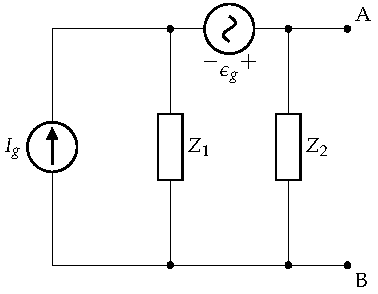
\includegraphics{../figs/Thevenin3}
\end{center}

Datos:
\begin{align*}
  \overline{\epsilon_g} &= \SI[parse-numbers=false]{32 + 12j}{\volt}\\
  \overline{I} &= \SI[parse-numbers=false]{2\phase{0}}{\ampere}\\
  \overline{Z}_1 &= \SI[parse-numbers=false]{8 - 6j}{\ohm}\\
  \overline{Z}_2 &= \SI[parse-numbers=false]{8 + 6j}{\ohm}
\end{align*}

\noindent\hrulefill

\subsection*{Solución}

Para obtener el generador dejamos el circuito en abierto y transformamos el generador de corriente en fuente de tensión. En el circuito resultante calculamos la corriente:

\begin{equation*}
  \overline{I} = \frac{\overline{\epsilon}_g + \overline{\epsilon}_1}{\overline{Z}_1 + \overline{Z}_2} = 3\phase{\ang{0}}\si{\ampere} 
\end{equation*}

Con esta corriente podemos calcular la tensión en la impedancia $Z_2$:

\begin{equation*}
  \overline{U}_{AB} = \overline{I} \cdot \overline{Z}_2 = 24 + 18j = 30\phase{\ang{36.87}}\si{\volt} = \overline{\epsilon}_{th}
\end{equation*}

Para obtener la impedancia apagamos las fuentes independientes. La impedancia vista desde AB es:

\begin{equation*}
  \overline{Z}_{AB} = \overline{Z}_1 || \overline{Z}_2 = 6.25\phase{\ang{0}}\si{\ohm} = \overline{Z}_{th}
\end{equation*}


\clearpage

\section{}

Obtén el generador equivalente de Thévenin del circuito de la figura respecto de A y B.
\begin{center}
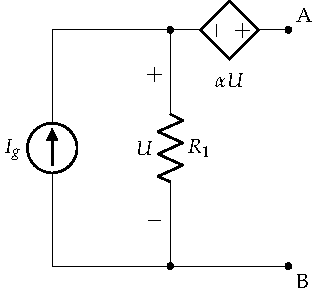
\includegraphics{../figs/Thevenin1}
\end{center}

\noindent\hrulefill

\subsection*{Solución}

Por una parte:

\begin{equation*}
  U_{AB} = \alpha U + U = (1 + \alpha) U
\end{equation*}

Además,

\begin{equation*}
  U = I_g \cdot R_1
\end{equation*}

Por tanto:

\begin{equation*}
  U_{AB} = (1 + \alpha) I_g R_1 = \epsilon_{th}
\end{equation*}

Para calcular la impedancia apagamos la fuente independiente. Como la fuente dependiente permanece, es necesario aplicar un generador de prueba a la salida.

\begin{minipage}{0.5\linewidth}
  \begin{center}
    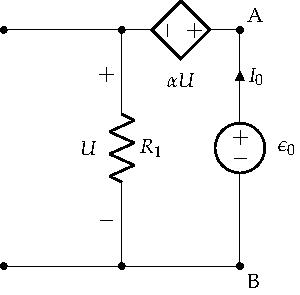
\includegraphics{../figs/Thevenin1_fuenteprueba}
  \end{center}
\end{minipage}
\begin{minipage}{0.5\linewidth}
  \begin{align*}
    \epsilon_0 &= (1 + \alpha) U\\
    U &= I_0 R_1
  \end{align*}
\end{minipage}
Por tanto,

\begin{equation*}
  Z_{th} = \frac{\epsilon_0}{I_0} = (1 + \alpha) R_1
\end{equation*}

\clearpage

\section{}

Obtén el generador equivalente de Thévenin del circuito de la figura respecto de A y B.

\begin{center}
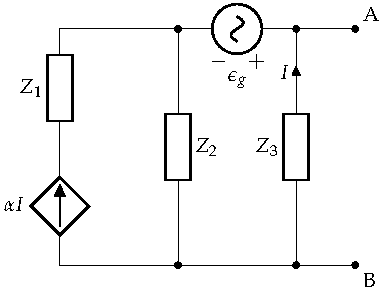
\includegraphics{../figs/Thevenin4}
\end{center}

Datos:
\begin{align*}
  \overline{\epsilon_g} &= \SI[parse-numbers=false]{12 - 16j}{\volt}\\
  \overline{Z}_1 &= \SI[parse-numbers=false]{1 - j}{\ohm}\\
  \overline{Z}_2 &= \SI[parse-numbers=false]{1 + j}{\ohm}\\
  \overline{Z}_3 &= \SI[parse-numbers=false]{5 + 3j}{\ohm}\\
  \alpha &= 2
\end{align*}

\noindent\hrulefill

\subsection*{Solución}

Dejamos el circuito en abierto y calculamos la tensión en AB:

\begin{align*}
  \overline{U}_{AB} &= \overline{\epsilon}_g + (1 + \alpha) \overline{I} \cdot \overline{Z}_2\\
  \overline{U}_{AB} &= - \overline{I} \cdot \overline{Z}_3
\end{align*}

Combinando estas ecuaciones obtenemos la tensión:

\begin{equation*}
  \overline{\epsilon}_{th} = \overline{U}_{AB} = \frac{\overline{\epsilon}_g}{1 + (1 + \alpha) \frac{\overline{Z}_2}{\overline{Z}_3}} = 6 - 10j = 11.66\phase{\ang{-59.04}}\si{\volt}
\end{equation*}

Para obtener la impedancia apagamos las fuentes independientes. Como hay fuentes dependientes debemos aplicar una fuente de prueba a la salida del circuito, con fuerza electromotriz $\overline{\epsilon}_0$ y corriente inyectada $\overline{I}_0$.

\begin{minipage}{0.5\linewidth}
  \begin{center}
    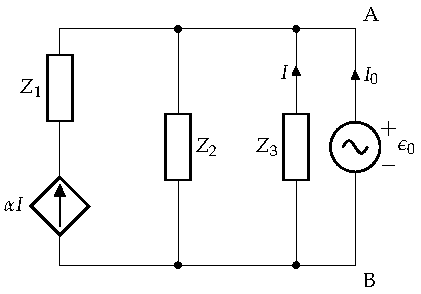
\includegraphics{../figs/Thevenin4_fuenteprueba}
  \end{center}
\end{minipage}
\begin{minipage}{0.5\linewidth}
  \begin{align*}
    \overline{\epsilon}_0 &= [(1 + \alpha) \overline{I} + \overline{I}_0] \cdot \overline{Z}_2\\
    \overline{\epsilon}_0 &= - \overline{I}\cdot \overline{Z}_3
  \end{align*}
\end{minipage}

Combinando ambas expresiones obtenemos:

\begin{equation*}
  \overline{Z}_{th} = \frac{\overline{\epsilon}_0}{\overline{I}_0} = \frac{\overline{Z}_2 \cdot \overline{Z}_3}{(1 + \alpha) \overline{Z}_2 + \overline{Z}_3} = 0.64 + 0.52j\si{\ohm}
\end{equation*}

Para obtener la máxima potencia disponible hay que conectar una impedancia:
\begin{equation*}
\overline{Z}_L = \overline{Z}^*_{th} = 0.64-0.52j\si{\ohm}
\end{equation*}

Esta impedancia disipará una potencia:
\begin{equation*}
P_L = \frac{\epsilon_{th}^2}{4 \cdot R_{th}} = \SI{53.11}{\watt}
\end{equation*}

\clearpage

\section{}

Obtén el generador equivalente de Thévenin del circuito de la figura respecto de A y B. A partir de este generador, calcula la resistencia a colocar en AB para obtener la máxima potencia, calculando esta potencia y la potencia entregada por el generador $\epsilon$.

\begin{center}
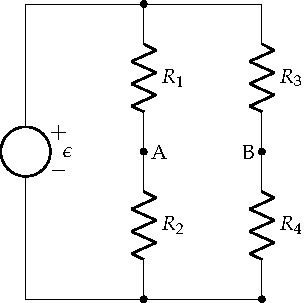
\includegraphics{../figs/Thevenin2}
\end{center}

Datos:

\begin{align*}
  \epsilon &= \SI{54}{\volt}\\
  R_1 = R_4 &= \SI{8}{\ohm}\\
  R_2 = R_3 &= \SI{10}{\ohm}
\end{align*}

\noindent\hrulefill

\subsection*{Solución}

Para obtener la tensión $U_{AB}$ aplicamos divisor de tensión en ambas ramas:

\begin{align*}
  U_A &= \epsilon \cdot \frac{R_2}{R_1 + R_2}\\
  U_B &= \epsilon \cdot \frac{R_4}{R_3 + R_4}\\
  U_{AB} &= \epsilon \cdot (\frac{R_2}{R_1 + R_2} -  \frac{R_4}{R_3 + R_4}) = \SI{6}{\volt} = \epsilon_{th}
\end{align*}

Para calcular la resistencia equivalente apagamos la fuente de tensión. En el circuito resultante obtenemos:

\begin{equation*}
  R_{th} = (R_1 || R_2) + (R_3 || R_4) = 80/9\si{\ohm}
\end{equation*}

Para obtener la máxima potencia hay que conectar una resistencia $R_L = R_{th}$. Con esta resistencia el balance de potencias es:

\begin{align*}
  P_L &= \frac{\epsilon_{th}^2}{4R_{th}} = \SI{1.0125}{\watt}\\
    P_\epsilon &= 2 \cdot P_L = \SI{2.025}{\watt}
\end{align*}

\clearpage

\section{}

Obtén el generador equivalente de Thévenin del circuito de la figura respecto de A y B. A partir de este generador, calcula la impedancia a colocar en AB para obtener la máxima potencia, calculando esta potencia.

\begin{center}
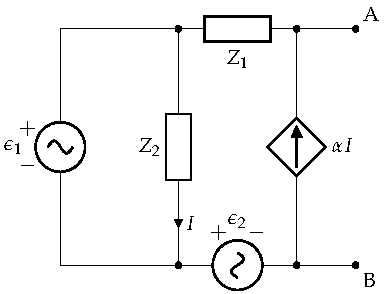
\includegraphics{../figs/Thevenin5}
\end{center}

Datos:
\begin{align*}
  \overline{\epsilon_1} &= \SI[parse-numbers=false]{10\phase{0}}{\volt}\\
  \overline{\epsilon_2} &= \SI[parse-numbers=false]{10j}{\volt}\\
  \overline{Z}_1 &= \SI[parse-numbers=false]{4 - 3j}{\ohm}\\
  \overline{Z}_2 &= \SI[parse-numbers=false]{3 + 4j}{\ohm}\\
  \alpha &= 2
\end{align*}

\noindent\hrulefill

\subsection*{Solución}

La tensión en circuito abierto es:

\begin{equation*}
  \overline{U}_{AB} = \alpha \overline{I} \cdot \overline{Z}_1 + \overline{\epsilon}_1 + \overline{\epsilon}_2
\end{equation*}
siendo $\epsilon_1 = \overline{Z}_2 \cdot \overline{I}$. Por tanto,

\begin{equation*}
  \epsilon_{th} = \alpha \cdot \overline{\epsilon}_1 \cdot \frac{\overline{Z}_1}{\overline{Z}_2} + \overline{\epsilon}_1 + \overline{\epsilon}_2 = 10 - 10j \si{\volt}
\end{equation*}

Para obtener la impedancia apagamos las fuentes independientes. Al apagar la fuente $\epsilon_1$, la impedancia $Z_2$ queda cortocircuitada y, por tanto, $I = 0$. En consecuencia, la fuente dependiente también queda apagada y obtenemos:

\begin{equation*}
  \overline{Z}_{th} = \overline{Z}_1 = 4 - 3j \si{\volt}
\end{equation*}

Para obtener la máxima potencia debemos conectar la impedancia:

\begin{equation*}
  \overline{Z}_{L} = \overline{Z}^*_{th} = 4 + 3j \si{\volt}
\end{equation*}

El balance de potencias es:

\begin{align*}
  P_L &= \frac{\epsilon_{th}^2}{4 \cdot R_{th}} = \SI{12.5}{\watt}\\
  P_{\epsilon} &= 2 \cdot P_L = \SI{25}{\watt} 
\end{align*}


\clearpage

\section{}

En el circuito de la figura calcula:

\begin{enumerate}
\item La fuerza electromotriz del generador equivalente de Thévenin respecto de A y B,  \(\overline{\epsilon_{th}}\).
\item La impedancia del generador equivalente de Thévenin respecto de A y B, \(\overline{Z_{th}}\).
\item La impedancia de carga que se debe conectar entre A y B para conseguir la máxima potencia disponible.
\item La potencia activa entregada entre A y B cuando se conecta cada una de las siguientes impedancias de carga. Comenta los resultados obtenidos.
\begin{itemize}
\item \(\overline{Z_L} = \overline{Z_{th}}\).
\item \(\overline{Z_L} = R_{th}\) (parte resistiva de \(\overline{Z_{th}}\)).
\item \(\overline{Z_L} = j X_{th}\) (parte reactiva de \(\overline{Z_{th}}\)).
\item Impedancia calculada en el apartado 3.
\end{itemize}
\end{enumerate}

\begin{minipage}{0.3\linewidth}
Datos:
\[
\overline{Z}_1 = 3 + j4\Omega
\]

\[
\overline{Z}_2 = 2 + j\Omega
\]

\[
\overline{\epsilon}_g = 10\angle 30^{\circ} V 
\]

\[
\overline{I}_g = 2\angle 15^{\circ} A
\]

\[
\beta = 5 \Omega
\]
\end{minipage}
\begin{minipage}{0.7\linewidth}
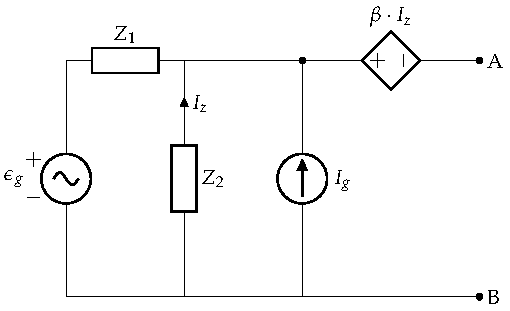
\includegraphics[width=.9\linewidth]{../figs/thevenin6.pdf}
\end{minipage}

\noindent\hrulefill

\subsection*{Solución}

Calculamos la tensión en circuito abierto, planteando las siguientes ecuaciones:

\begin{align*}
  \overline{I}_g + \overline{I}_Z + \overline{I}_{Z1} &= 0\\
  - \overline{I}_Z \cdot \overline{Z}_2 &= \overline{\epsilon}_g - \overline{I}_{Z1} \cdot \overline{Z}_1\\
  \overline{U}_{AB} = - \beta \cdot \overline{I}_Z - \overline{I}_Z \cdot \overline{Z}_2
\end{align*}

Combinando estas ecuaciones obtenemos:

\begin{equation*}
  \overline{U}_{AB} = (\beta + \overline{Z}_2) \cdot \frac{\overline{\epsilon}_g + \overline{I}_g \cdot \overline{Z}_1}{\overline{Z}_1 + \overline{Z}_2} = 138.48 + 3.99j \si{\volt} = \overline{\epsilon}_{th}
\end{equation*}

Para calcular la impedancia apagamos las fuentes independientes y conectamos un generador de prueba en AB:

\begin{minipage}{0.5\linewidth}
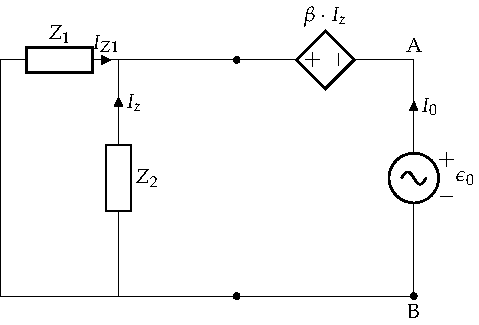
\includegraphics[width=.9\linewidth]{../figs/thevenin6_fuenteprueba.pdf}
\end{minipage}
\begin{minipage}{0.5\linewidth}
  \begin{align*}
    \overline{I}_0 + \overline{I}_Z + \overline{I}_{Z1} &= 0\\
    \overline{I}_Z \cdot \overline{Z}_2 &= \overline{I}_{Z1} \cdot \overline{Z}_1\\
    \overline{\epsilon}_0 &= - \beta \cdot \overline{I}_Z - \overline{I}_Z \cdot \overline{Z}_2
  \end{align*}
\end{minipage}
Por tanto,

\begin{equation*}
  \overline{Z}_{th} = \frac{\overline{\epsilon}_0}{\overline{I}_0} = \frac{\beta + \overline{Z}_2}{1 + \overline{Z}_2/\overline{Z}_1} = 4.8 + 1.4j\si{\ohm}
\end{equation*}

La potencia en AB depende de la carga conectada:

\begin{equation*}
  P_{AB} = R_L \cdot \frac{\epsilon_{th}^2}{|\overline{Z}_L + \overline{Z}_{th}|^2}
\end{equation*}

\begin{itemize}
\item Cuando $\overline{Z}_L = \overline{Z}_{th}$, $P_{AB} = \SI{17.15}{\watt}$
\item Cuando $\overline{Z}_L = R_{th}$, $P_{AB} = \SI{18.22}{\watt}$
\item Cuando $\overline{Z}_L = jX_{th}$, $P_{AB} = \SI{0}{\watt}$
\item Cuando $\overline{Z}_L = \overline{Z}^*_{th}$, $P_{AB} = \SI{18.61}{\watt}$
\end{itemize}

Comprobamos que el máximo valor se obtiene cuando conectamos la impedancia de Thévenin conjugada.

\clearpage

\section{}

En el circuito de la figura calcula:

\begin{enumerate}
\item La corriente del generador equivalente de Norton respecto de A y B, $I_N$.
\item La resistencia del generador equivalente de Norton respecto de A y B, $R_N$.
\item La resistencia de carga que se debe conectar entre A y B para conseguir la máxima potencia disponible, y el valor de esta potencia.
\end{enumerate}

\begin{minipage}{0.3\linewidth}
Datos:
\[
  R = \SI{1}{\ohm}
\]

\[
\epsilon_g = \SI{10}{\volt}
\]

\[
  \alpha = \beta = 1
\]

\end{minipage}
\begin{minipage}{0.7\linewidth}
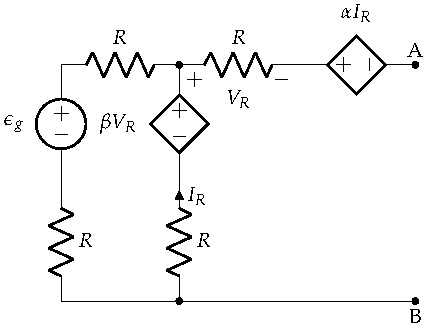
\includegraphics[width=.9\linewidth]{../figs/norton.pdf}
\end{minipage}

\subsection*{Solución}

Para calcular el equivalente de Norton cortocircuitamos la salida del circuito. Podemos escribir las siguientes ecuaciones:

\begin{minipage}{0.5\linewidth}
  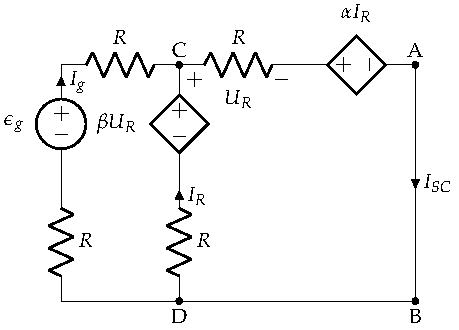
\includegraphics[width=.9\linewidth]{../figs/norton_corto.pdf}
\end{minipage}
\begin{minipage}{0.5\linewidth}
  \begin{align*}
    U_R &= R \cdot I_{sc}\\
    I_g+ I_R &= I_{sc}\\
    U_{CD} &= \epsilon_g - 2 \cdot R \cdot I_g\\
    U_{CD} &= \beta \cdot U_r - I_R \cdot R\\
    U_{CD} &= U_R + \alpha \cdot I_R
  \end{align*}
\end{minipage}

Combinando estas ecuaciones obtenemos:

\begin{equation*}
  I_{sc} = 10/3\si{\ampere} = I_N
\end{equation*}

Para obtener la resistencia equivalente apagamos la fuente independiente y conectamos un generador de prueba en AB:


\begin{minipage}{0.5\linewidth}
  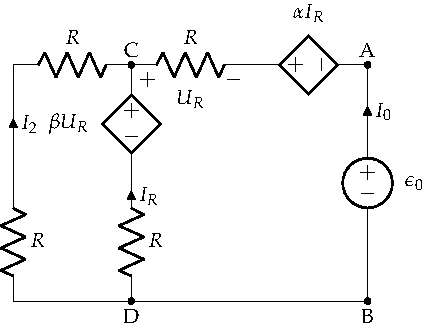
\includegraphics[width=.9\linewidth]{../figs/norton_fuenteprueba.pdf}
\end{minipage}
\begin{minipage}{0.5\linewidth}
  \begin{align*}
    U_R &= -I_0 \cdot R\\
    I_2 + I_R + I_0 &= 0\\
    U_{CD} &= -2R\cdot I_2\\
    U_{CD} &= \beta \cdot U_R - I_R \cdot R\\
    U_{CD} &= U_R + \alpha \cdot I_R + \epsilon_0
  \end{align*}
\end{minipage}

Combinando estas ecuaciones obtenemos:

\begin{equation*}
  R_{th} = \frac{\epsilon_0}{I_0} = \SI{2}{\ohm}
\end{equation*}

Por tanto, habrá que conectar una resistencia de $\SI{2}{\ohm}$ para obtener la máxima potencia disponible.

\end{document}
